\chapter{Экспериментальная часть}

В данном разделе описаны проведённые замеры и представлены результаты исследования. Также будут уточнены характеристики устройства, на котором проводились замеры.

\section{Технические характеристики}
Технические характеристики устройства, на котором выполнялось тестирование \cite{web_item5}:
\begin{itemize}
	\item операционная система macOS Monterey 12.4;
	\item 8 ГБ оперативной памяти;
	\item процессор Apple M2 (базовая частота~---~2400 МГц, но поддержка технологии Turbo Boost позволяет достигать частоты в 3500 МГц \cite{web_item10}).
\end{itemize}

\section{Измерение времени выполнения реализаций алгоритмов}
Тестирование реализаций алгоритмов производилось при помощи встроенных в Go средств, а именно «бенчмарков» ($benchmarks$ из пакета $testing$ стандартной библиотеки $Go$ \cite{web_item3}), представляющих собой тесты производительности. По умолчанию производятся только замеры времени выполнения в наносекундах \cite{web_item11}\cite{web_item12}, но при добавлении ключа $-benchmem$ также выполняется замер потребления памяти и количества аллокаций памяти.

Значение $N$ динамически изменяется для достижения стабильного результата при различных условиях, но гарантируется, что каждый «бенчмарк» будет выполняться хотя бы одну секунду. Для замеров использовались массивы равной длины, генерирующиеся  различными способами, в зависимости от особенностей худших и лучших случаев для алгоритмов, перед началом выполнения «бенчмарков». Результаты тестирования возвращаются в структуре специального вида. Пример такой структуры представлен в листинге \ref{code:go_bench_struct}.

\begin{code}
\caption{Листинг структуры результата «бенчмарка»}
\label{code:go_bench_struct}

\begin{minted}{go}
testing.BenchmarkResult{N:120000, T:1200000000, Bytes:0, MemAllocs:0x0, 
MemBytes:0x0, Extra:map[string]float64{}}
\end{minted}
\end{code}

В листинге \ref{code:go_bench} представлен пример реализации «бенчмарка», где $alg.function$~---~объект типа функция (в данной реализации~---~функция, описывающая один из алгоритмов сортировки).
\begin{code}
\caption{Листинг примера реализации «бенчмарка»}
\label{code:go_bench}
\begin{minted}{go}
func NewBenchmark(arr []int, alg algorithm) func(*testing.B) {
	return func(b *testing.B) {
		copyA := make([]int, len(arr))
		b.ResetTimer()
		for j := 0; j < b.N; j++ {
			b.StopTimer()
			copy(copyA, arr)
			b.StartTimer()
			alg.function(copyA)
		}
	}
}
\end{minted}
\end{code}

Входные массивы для проведения замеров генерируются следующими способами:
\begin{itemize}
	\item генерация случайных чисел в диапазоне от 1 до значения длины массива;
	\item заполнение числами от 1 до значения длины массива в порядке возрастания;
	\item заполнение числами от 1 до значения длины массива в порядке убывания;
	\item заполнение одним значением;
	\item заполнение с чередованием элементов по величине.
\end{itemize}

Пример функции для генерации массива представлен в листинге \ref{code:gen}.

\newpage

\begin{code}
\caption{Листинг примера функции для генерации массива с заполнением случайными числами в диапазоне от 1 до значения длины массива}
\label{code:gen}
\begin{minted}{go}
func generateArray(size int) []int {
	rand.Seed(time.Now().UnixNano())
	
	arr := make([]int, 0, size)
	for j := 0; j < size; j++ {
		arr = append(arr, rand.Intn(size)+1)
	}

	return arr
}
\end{minted}
\end{code}

\newpage

Результаты замеров времени выполнения (в нс.) приведены в таблицах \ref{table:sort_time1}~---~\ref{table:sort_time3}. На рисунках \ref{img:graph1}~---~\ref{img:graph3} приведены графики, отображающие зависимость времени работы алгоритмов от длины массива для произвольного, лучшего и худшего случаев. Массивы заполнялись случайными числами.

\begin{table}[H]
  \caption{\label{table:sort_time1} Результаты замеров времени для произвольного случая (нс.)}
  \begin{center}
    \begin{tabular}{
    |S[table-format=4.0]
    |S[table-format=10.0]
    |S[table-format=10.0]
    |S[table-format=10.0]|
    }
      \hline
      {Длина массива} & {Блинная} & {Быстрая} & {Бусинами} \\ \hline
      1 & 50 & 452 & 508\\ \hline
      10 & 224 & 1701 & 2067\\ \hline
      50 & 2594 & 8156 & 16532\\ \hline
      100 & 9898 & 12416 & 48092\\ \hline
      200 & 40020 & 25810 & 247140\\ \hline
      300 & 87373 & 34310 & 782144\\ \hline
      500 & 230788 & 59792 & 2566986\\ \hline
      600 & 326217 & 67896 & 2606156\\ \hline
      800 & 568568 & 98698 & 4774437\\ \hline
      1000 & 874516 & 127788 & 11649473\\ \hline
    \end{tabular}
  \end{center}
\end{table}

\noindent
\begin{table}[h!]
  \centering
  \begin{tabular}{p{1\linewidth}}
    \centering
    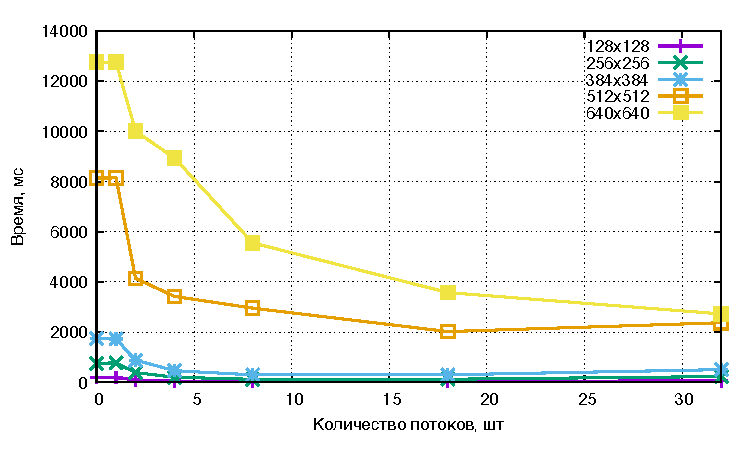
\includegraphics[width=0.8\linewidth]{../data/time.pdf}
    \captionof{figure}{Зависимость времени работы алгоритмов сортировки от длины массива}
    \label{img:graph1}
  \end{tabular}
\end{table}

\begin{table}[H]
  \caption{\label{table:sort_time2} Результаты замеров времени для лучшего случая (нс.)}
  \begin{center}
    \begin{tabular}{
    |S[table-format=4.0]
    |S[table-format=10.0]
    |S[table-format=10.0]
    |S[table-format=10.0]|
    }
      \hline
      {Длина массива} & {Блинная} & {Быстрая} & {Бусинами} \\ \hline
      1 & 51 & 326 & 516\\ \hline
      10 & 131 & 1476 & 928\\ \hline
      50 & 1690 & 5718 & 1972\\ \hline
      100 & 5658 & 9916 & 3518\\ \hline
      200 & 21382 & 17774 & 5847\\ \hline
      300 & 47410 & 26439 & 8335\\ \hline
      500 & 130256 & 41003 & 12737\\ \hline
      600 & 186585 & 51371 & 16124\\ \hline
      800 & 330680 & 70031 & 20843\\ \hline
      1000 & 515007 & 84321 & 25283\\ \hline
    \end{tabular}
  \end{center}
\end{table}

\noindent
\begin{table}[h!]
  \centering
  \begin{tabular}{p{1\linewidth}}
    \centering
    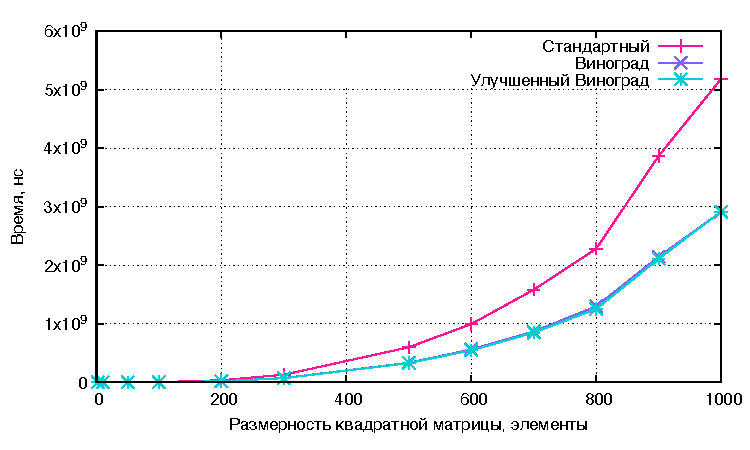
\includegraphics[width=0.8\linewidth]{../data/time_best.pdf}
    \captionof{figure}{Зависимость времени работы алгоритмов сортировки от длины массива}
    \label{img:graph2}
  \end{tabular}
\end{table}

\begin{table}[H]
  \caption{\label{table:sort_time3} Результаты замеров времени для худшего случая (нс.)}
  \begin{center}
    \begin{tabular}{
    |S[table-format=4.0]
    |S[table-format=10.0]
    |S[table-format=10.0]
    |S[table-format=10.0]|
    }
      \hline
      {Длина массива} & {Блинная} & {Быстрая} & {Бусинами} \\ \hline
      1 & 52 & 272 & 528\\ \hline
      10 & 258 & 2085 & 2654\\ \hline
      50 & 3209 & 16191 & 17435\\ \hline
      100 & 12278 & 38466 & 57557\\ \hline
      200 & 47484 & 122015 & 432274\\ \hline
      300 & 103360 & 241772 & 1295117\\ \hline
      500 & 278107 & 683739 & 4296667\\ \hline
      600 & 394568 & 879124 & 5070336\\ \hline
      800 & 693190 & 1549153 & 7614436\\ \hline
      1000 & 1074233 & 2262414 & 20137148\\ \hline
    \end{tabular}
  \end{center}
\end{table}

\noindent
\begin{table}[h!]
  \centering
  \begin{tabular}{p{1\linewidth}}
    \centering
    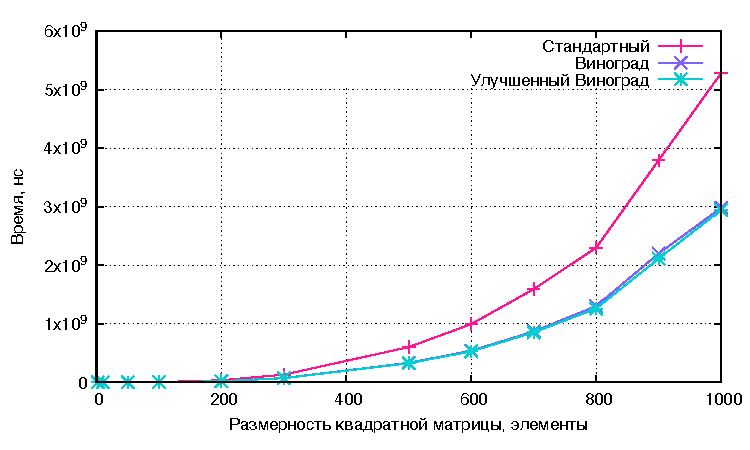
\includegraphics[width=0.8\linewidth]{../data/time_worst.pdf}
    \captionof{figure}{Зависимость времени работы алгоритмов сортировки от длины массива}
    \label{img:graph3}
  \end{tabular}
\end{table}

\section{Измерение объёма потребляемой памяти реализаций}
Измерение объёма потребляемой памяти производилось посредством создания собственного программного модуля memory, использующего функции пакета unsafe языка $Go$ \cite{web_item3}. Реализация основного функционала модуля, а также пример функции расчёта памяти, затрачиваемой на алгоритм блинной сортировки, и пример использования указанных функций приведены в Приложении А.

Результаты замеров потребляемой памяти (в байтах) приведены в таблице \ref{table:sort_mem}. На рисунке \ref{img:graph4} приведён график, отображающий зависимость потребляемой памяти от длины массива. Массивы заполнялись случайными числами.

\begin{table}[h]
  \caption{\label{table:sort_mem} Результаты замеров потребляемой памяти (в байтах)}
  \begin{center}
    \begin{tabular}{
    |S[table-format=4.0]
    |S[table-format=10.0]
    |S[table-format=10.0]
    |S[table-format=10.0]|
    }
      \hline
      {Длина массива} & {Блинная} & {Быстрая} & {Бусинами} \\ \hline
      1 & 128 & 176 & 168\\ \hline
      10 & 128 & 1232 & 384\\ \hline
      50 & 128 & 3176 & 4544\\ \hline
      100 & 128 & 4872 & 64944\\ \hline
      200 & 128 & 11208 & 160144\\ \hline
      300 & 128 & 12320 & 72144\\ \hline
      500 & 128 & 16816 & 1372144\\ \hline
      600 & 128 & 20184 & 2380944\\ \hline
      800 & 128 & 31896 & 1043344\\ \hline
      1000 & 128 & 35896 & 712144\\ \hline
    \end{tabular}
  \end{center}
\end{table}

\newpage

\noindent
\begin{figure}[t!]
	\centering
    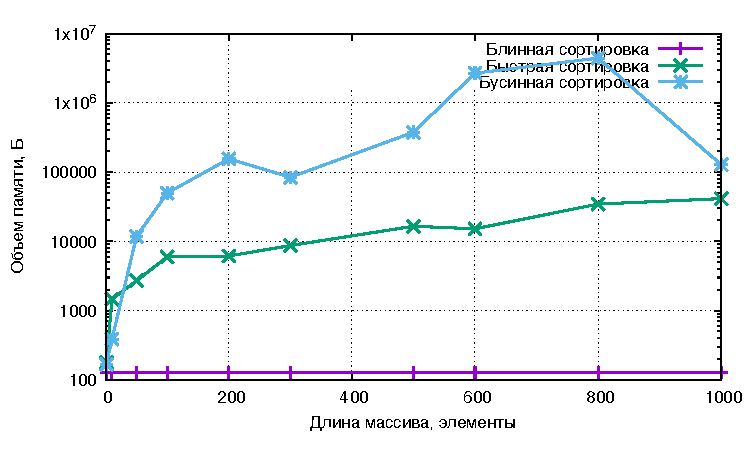
\includegraphics[width=0.95\linewidth]{../data/memory.pdf}
    \caption{Зависимость потребляемой памяти при сортировке от длины массива}
    \label{img:graph4}
\end{figure}

\newpage